\chapter{Vorbetrachtungen}

\section{Allgemeine Softwareentwicklung}
\label{sec:allgemeine_softwareentwicklung}

In dieser Arbeit soll der Begriff Softwareentwicklung den Prozess benennen, der alle Aktivit"aten und die damit verbundenen (Zwischen-) Ergebnisse bei der Erstellung von Software umfasst.
In der Literatur wird auch der Begriff Softwareprozess genutzt \cite{Sommerville2001a}.
Obwohl verschiedene Vorgehensmodelle f"ur das Erstellen von Software existieren, haben alle Softwareentwicklungsprozesse vier grundlegende Arbeitsaktivit"aten gemeinsam \cite{Brugge2004a,Sommerville2001a}:
\begin{description}
	\item[Softwarespezifikation:] Es m"ussen die konkreten Anforderungen an das zu erstellende Programm ermittelt werden.
								  Dabei wird die Funktion der Software, aber auch die Grenzen der Benutzung definiert.
	\item[Softwareentwurf und -implementierung:] Nach Analyse der ermittelten Anforderungen kann die Architektur des Softwaresystems entworfen werden.
												 Durch die Zerlegung der Software in mehrere Subsysteme werden die Anforderungen in kleine Teilprobleme aufgeteilt.
												 Diese Teilprobleme sind den verschiedenen Komponenten und Objekten der Software zugeordnet und k"onnen seperat gel"ost werden.
												 Diese L"osung wird durch den Objektentwurf und die schlu\ss endliche Implementierung des jeweiligen Programmteils erreicht.
	\item[Validierung der Software:] Die fertige Software muss auf ihre Funktionsf"ahigkeit "uberpr"uft werden.
									 Hierbei ist auch abzusichern, dass die Software neben der gew"unschten Funktionalit"at keine ungewollten Nebeneffekte auftreten.
	\item[Weiterentwicklung:] Ein Programm muss sich im Laufe seiner Lebenszeit weiter entwickeln um den sich "andernden Nutzeranforderungen gerecht zu werden.
\end{description}

Der Punkte der Softwarespezifikation ist im \chapref{spezifikation} abgehandelt.
Im \chapref{entwurf} wird neben der Struktur und dem Aufbau des Programms auch auf die Fragen bez"uglich Entwurfsentscheidungen eingegangen.
Durch die Validierung der Software muss sicher gestellt werden, dass die Software die Erwartungen des Benutzers erf"ullt und den an sie gestellten Bedingungen gerecht wird.
Dieser Punkt ist im \secref{testszenarien} behandelt.
Zudem muss das Programm auch schon w"ahrend der Entwicklung immer wieder auf die korrekte Funktionsweise "uberpr"uft werden.
Dazu wird auch auf Tests der einzelnen Komponenten in den jeweilegen Abschnitten im \chapref{entwurf} eingegangen.
Der letzte der vier oben genannten Aspekte ist in dieser Arbeit ein nicht zu vernachl"assigender Punkt.
Weil gerade das Programm f"ur die Nutzung w"ahrend der Entwicklung von Signalverarbeitungsmethoden erstellt wird, werden die Anforderungen an das Programm fortlaufend wachsen.
Somit soll schon von Beginn an die Erweiterbarkeit dieses Projektes unterst"utzt und gef"ordert werden.
Deshalb sind auch in den folgenden Anforderungen Punkte enthalten die diesen Aspekt besonders hervorheben und explizit fordern.

\begin{figure}[htb]
\centering
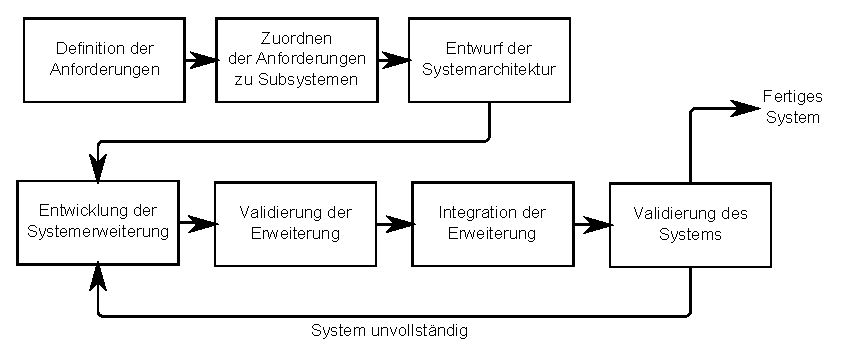
\includegraphics[width=0.9\textwidth]{bilder/inkrementelle_entwicklung.eps}
\caption{Inkrementeller Softwareentwicklungsansatz nach \cite{Sommerville2001a}}
\label{pic:inkrementelle_entwicklung}
\end{figure}
F"ur die in dieser Arbeit zu entwickelnden Sofware wird eine Methode der inkrementellen Entwicklung genutzt.
Die Herangehensweise dieser Methode ist in \picref{inkrementelle_entwicklung} dargestellt.
Nach der anf"anglichen Feststellung und Definition der grundlegenden Anforderungen an die zu programmierende Software, wird die allgemeine Struktur des Programms festgelegt.
Die Subkomponenten des Programms werden einzeln entworfen und in das bestehende Programm integriert.
Da die neuen Subkomponenten immer Teilanforderungen des Programmes erf"ullen, steigert sich somit die Funktionalit"at des Programms.
Dieser Ansatz hat den Vorteil, dass die Software schon zeitig im Entwicklungsstadium getestet werden kann und damit auch schon Erfahrungen gesammelt werden k"onnen.
Zus"atzlich k"onnen gew"unschte "Anderungen der Bedienung oder der Funktionalit"at erkannt und implementiert werden.

%-- konkrete auf Schritte der Softwarespezifikation eingehen
%-- details "uber vorgehen bei der Implementierung
%-- anmerkungen f"ur Test der Komponenten und des Gesamtprogrammes
%Theorie zu Softwareentwurf
%-- Anforderungen: funktional und nichtfunktional
%-- Weiterentwicklung



\section{[WIP]Genutzte Biosignale zur Programmvalidierung}
\label{sec:genutzte_biosignale}

%\begin{wrapfigure}{r}{0.5\textwidth}
\begin{figure}
	\centering
	\includegraphics[width=0.6\textwidth]{bilder/elektroden_konfiguration.pdf}
	\caption[Elektrodenkonfiguration zur Aufnahme des abdominalen \ac{EKG}-Signals]{Elektrodenkonfiguration zur Aufnahme des abdominalen \ac{EKG}-Signals \cite{Zaunseder2012}}
	\label{pic:elektroden_konfig}
\end{figure}
%\end{wrapfigure}

F"ur die Validierung des Programmes werden typische Arbeitsschritte mit dem Programm auf Beispieldatens"atze durchgef"uhrt.
In diesem Abschnitt soll kurz die genutzten Daten n"aher beschrieben werden.

\subsection{Abdominale \aclp{EKG}}

F"ur Untersuchungen von \ac{EKG}-Daten von Feten werden \acp{EKG} von Schwangeren abdominal aufgenommen.
Die Datenaufzeichnung f"ur das \ac{IBMT} erfolgt in Zusammenarbeit der Abteilung f"ur Pr"anatal- und Geburtsmedizin der Universit"atsklink Leipzig.
Daf"ur werden die \acp{EKG} mit sieben Kan"alen aufgezeichnet (Elektrodenkonfiguration zwei bis acht in \picref{elektroden_konfig}).
Die Aufzeichnungsdauer betr"agt rund 20 Minuten und die Daten werden mit $1{}kHz$ abgetastet.
Weitere Details "uber die Datenaufzeichnung und der Datenverarbeitung sind in den Arbeiten von F. Andreotti \cite{Andreotti2011}, M. C. Santiago \cite{Santiago2012} und S. Zaunseder \cite{Zaunseder2012} beschrieben.
%-- abdmECG Schwangerer
%-- aufgenommen durch Projektpartner in Leipzig (Universit"atsfrauenklinik Leipzig / Institut f"ur Geburtshilfe und Gyn"akologie)
%-- 7 kan"ale: 2-8 aus \cite{Zaunseder2012}
%-- Datensatz enth"alt: 
Die f"ur die Validierung genutzten Datens"atze enthalten folgende Elemente:
\begin{itemize}
	\item Rohdaten (sieben Kan"ale)
	\item vorverarbeitete Daten (gefilterte Rohsignale mit einem Bandpass (Durchlassbereich $2$ bis $100{}Hz$ \cite{Andreotti2011}) und einem $49-51{}Hz$-Notchfilter)
	\item Absch"atzung der m"utterlichen und fetalen \acp{EKG}
	\item Detektionen der m"utterlichen und fetalen QRS-Komplexe (als Annotationen)
	\item m"utterliche und fetale RR-Zeitreihen aus der QRS-Detektion abgeleitet
\end{itemize}
Insgesamt enth"alt ein jeder Datensatz 28 Kan"ale \ac{EKG}-Daten, 14 Annotationskan"ale und 14 RR-Zeiteihen.
Eine Kontrolle der automatisierten QRS-Detektion ist in diesem Fall notwendig, da die Detektionsrate zwischen $66,1$ und $94,5{}\%$ \cite{Zaunseder2012} schwankt.
%-- Annotation notwendig zur Kontrolle der automatisiert detektierten QRS Komplexe, weil Detektionsrate stark schwankend ($66,1 - 94,5$\% \cite{Zaunseder2012})



\subsection{[WIP]Videogest"utzte Herzratenermittlung}


-- Teil von Cui Zhai \cite{Zhai2012}:
\begin{itemize}
	\item \ac{EKG}
	\item \ac{PPG}
	\item RR-Intervalle (\ac{hrv}, aus obigen abgeleitet)
\end{itemize}


%% EOF %%%%%%%%%%%%%%%%%%%%%%%%%%%%%%%%%%%%%%%%%%%%%%%%%%%%%%
